\documentstyle[12pt,aaspp4]{article}


%%%%%%%%%%%%%%%%%%%%%%%%%%%%%%%%%%%%%%%%%%%%%%%%%%%%
%%% author-defined commands
\newcommand\about     {\hbox{$\sim$}}
\newcommand\x         {\hbox{$\times$}}
\newcommand\othername {\hbox{$\dots$}}
\def\eq#1{\begin{equation} #1 \end{equation}}
\def\eqarray#1{\begin{eqnarray} #1 \end{eqnarray}}
\def\eqarraylet#1{\begin{mathletters}\begin{eqnarray} #1 %
                  \end{eqnarray}\end{mathletters}}
\def\non    {\nonumber \\}
\def\DS     {\displaystyle}
\def\E#1{\hbox{$10^{#1}$}}
\def\sub#1{_{\rm #1}}
\def\case#1/#2{\hbox{$\frac{#1}{#2}$}}
\def\about  {\hbox{$\sim$}}
\def\x      {\hbox{$\times$}}
\def\ug               {\hbox{$u-g$}}
\def\gr               {\hbox{$g-r$}}
\def\ri               {\hbox{$r-i$}}
\def\iz               {\hbox{$i-z$}}
\def\a                {\hbox{$a^*$}}
\def\O                {\hbox{$O$}}
\def\E                {\hbox{$E$}}
\def\Oa               {\hbox{$O_a$}}
\def\Ea               {\hbox{$E_a$}}
\def\Jg               {\hbox{$J_g$}}
\def\Fg               {\hbox{$F_g$}}
\def\J                {\hbox{$J$}}
\def\F                {\hbox{$F$}}
\def\N                {\hbox{$N$}}
\def\dd               {\hbox{deg/day}}
\def\mic              {\hbox{$\mu{\rm m}$}}
\def\Mo{\hbox{$M_{\odot}$}}
\def\Lo{\hbox{$L_{\odot}$}}
\def\comm#1           {\tt #1}
\def\refto#1          {\ref #1}
\def\T#1              {({\bf #1})}
\def\H#1              {({\it #1})}

%%%%%%%%%%%%%%%%%%%%%%%%%%%%%%%%%%%%%%%%%%%%%%%%%%%%

\begin{document}



\title{ {\bf Term Project \# 3}}  
                   
\centerline{Galactic Astronomy (Astr 511); Winter Quarter 2017}
\centerline{prof. Mario Juri\'{c} and prof. \v{Z}eljko Ivezi\'{c}, University of Washington} 

\section{Introduction} 


This homework is based on APOGEE-ASPCAP spectroscopic data\footnote{See http://www.sdss.org/dr12/irspec/}. 
We will use measured abundances for 15 elements (from the summary APOGEE-ASPCAP allStar file) and 
other data to study the variation of abundance distribution as a function of stellar population (halo,
thin disk, thick disk). 

Copying verbatim from the SDSS Data Release webpage\footnote{http://www.sdss.org/dr12/irspec/aspcap/},
``The APOGEE Stellar Parameters and Chemical Abundances Pipeline (ASPCAP) employs a two-step process 
to extract abundances: first, determination of the atmospheric parameters by fitting the entire APOGEE spectrum, 
and second, use of these parameters to fit various small regions of the spectrum dominated by spectral features
 associated with a particular element in order to derive the individual element abundance.''
The first ASPCAP step estimates seven stellar parameters: effective temperature, surface gravity, microturbulence, 
overall metal abundance $[M/H]$, relative $\alpha$-element abundance $[\alpha/M]$ (defined as O, Mg, Si, S, 
Ca, and Ti changing with solar proportions in lockstep), carbon $[C/M]$, and nitrogen $[N/M]$ abundances.
The second step estimates abundances of the following 15 elements: Al, Ca, C, Fe, K, Mg, Mn, Na, Ni, N, O, Si, S, Ti, and V.
The $[\alpha/Fe]$ value estimated during the first ASPCAP step and a corresponding value based on the
measured abundances of individual $\alpha$ elements (note that $\alpha$ elements Ne and Ar are missing): 
\begin{equation}
       [\alpha/Fe]^\ast= {[O/H]+[Mg/H]+[Si/H]+[S/H]+[Ca/H]+[Ti/H] \over 6} - [Fe/H],
\end{equation}
are in good agreement. In other words, $[\alpha/Fe]$ shows good correspondence to the {\it mean} value 
of the abundances of the above six elements, and the last term transforms the scale from ``per $H$'' to ``per $Fe$''. 

These stellar parameters and abundances (for 163,278 stars) are conveniently stored in a single 
fits\footnote{For data model, see https://data.sdss.org/datamodel/files/APOGEE\_REDUX/ \\
APRED\_VERS/APSTAR\_VERS/ASPCAP\_VERS/RESULTS\_VERS/allStar.html}
file; the Data Release 12 version\footnote{For download, see http://www.sdss.org/dr12/data\_access/bulk/} 
is named allStar-v603.fits (602 MB). If the data are read as 
\begin{verbatim}
data = pyfits.open('allStar-v603.fits')[1].data[::1] 
\end{verbatim}
then $[\alpha/Fe]$ from the first stage can be accessed as 
\begin{verbatim}
alphaFe = data['PARAM_ALPHA_M']
\end{verbatim}
while individual abundances can be accessed as, e.g. for Mg and Ti,
\begin{verbatim}
MgH = data['MG_H']
TiH = data['TI_H'].
\end{verbatim}
The overall metal abundance can be read as 
\begin{verbatim}
MH = data['PARAM_M_H']
\end{verbatim}
and $[Fe/H]$, 
\begin{verbatim}
FeH = data['Fe_H'].
\end{verbatim}

Using these data (for extra credit, use quality flags\footnote{See ASPCAP Bitmasks section at http://www.sdss.org/dr12/irspec/parameters/} too!) and 
\begin{enumerate}
\item Estimate the median difference and root-mean-square (rms) scatter of the difference between $[\alpha/Fe]$ and $[\alpha/Fe]^\ast$. Does the distribution of this difference appear Gaussian? Is the median difference correlated with T$_{eff}$, log(g), $[Fe/H]$, or $[\alpha/Fe]$? 
% a median of $-0.008$ dex and rms of 0.042 dex, 
\item Estimate the median difference and root-mean-square (rms) scatter of the difference between $[M/H]$ and $[Fe/H]$. 
Does the distribution of this difference appear Gaussian? 
Is the median difference correlated with T$_{eff}$, log(g), $[Fe/H]$, or $[\alpha/Fe]$? 
% a median of $0.007$ dex and rms of 0.077 dex, 
\item Plot the K vs. J$-$K color-magnitude Hess (pixelized) diagram and color code it by the mean log(g) per pixel.
Do you see any structure in the log(g) distribution (that is, is log(g) correlated with J-K or K)? If so, discuss and explain it. 
Note that this real data file also includes some outliers; the plausible ranges to be used in the plot are 0.0 to 4.0 for 
the J-K color and 14 to 6 for K magnitude (real astronomers plot magnitudes as decreasing along y axis; i.e. bright is up!). 
\item Plot log(g) vs. T$_{eff}$ Hess diagram and color code it by the mean $[Fe/H]$ per pixel.
Describe and explain the seen structure (hint: the gradient of $[Fe/H]$). Axes should be oriented so that 
this diagram resembles a standard Hertzsprung-Russell diagram.  
\item Plot $[\alpha/Fe]$ vs. $[Fe/H]$ Hess diagram and color code it by the mean log(g) per pixel.
Overplot contours showing the number of stars per pixel. Do you see any structure? If so, discuss and explain it. 
Hint: plot $[\alpha/Fe]$ histogram for a subsample with $-0.5 < [Fe/H] < -0.2$; is it Gaussian? 
\item Plot $[\alpha/Fe]$ vs. $[Fe/H]$ Hess diagram and color code it by the velocity dispersion (rms scatter) per pixel.
Overplot contours showing the number of stars per pixel. Do you any structure? If so, discuss and explain it. 
\item Now repeat the last step separately for stars with Galactic latitudes $|b| < 5^\circ$ and $|b| > 20^\circ$ and 
use the observed difference to discuss whether your previous answer makes sense.  
\end{enumerate}


Hint: the halo, thick disk and thin disk populations can be approximately defined as:
\begin{verbatim}
# define thin/thick/halo subsamples using [Fe/H] and [alpha/Fe] cuts
MH = data['PARAM_M_H']
alphaFe = data['PARAM_ALPHA_M']
condHalo = (MH > -2.5) & (MH < -1.1))
condDisk = (MH > -0.9) & (MH < 0.6))
condThin = (condDisk & (alphaFe > 0.0) & (alphaFe < 0.15)) 
condThick = (condDisk & (alphaFe > 0.15) & (alphaFe < 0.35)) 
\end{verbatim}


\end{document}



\begin{figure}
  \centering
  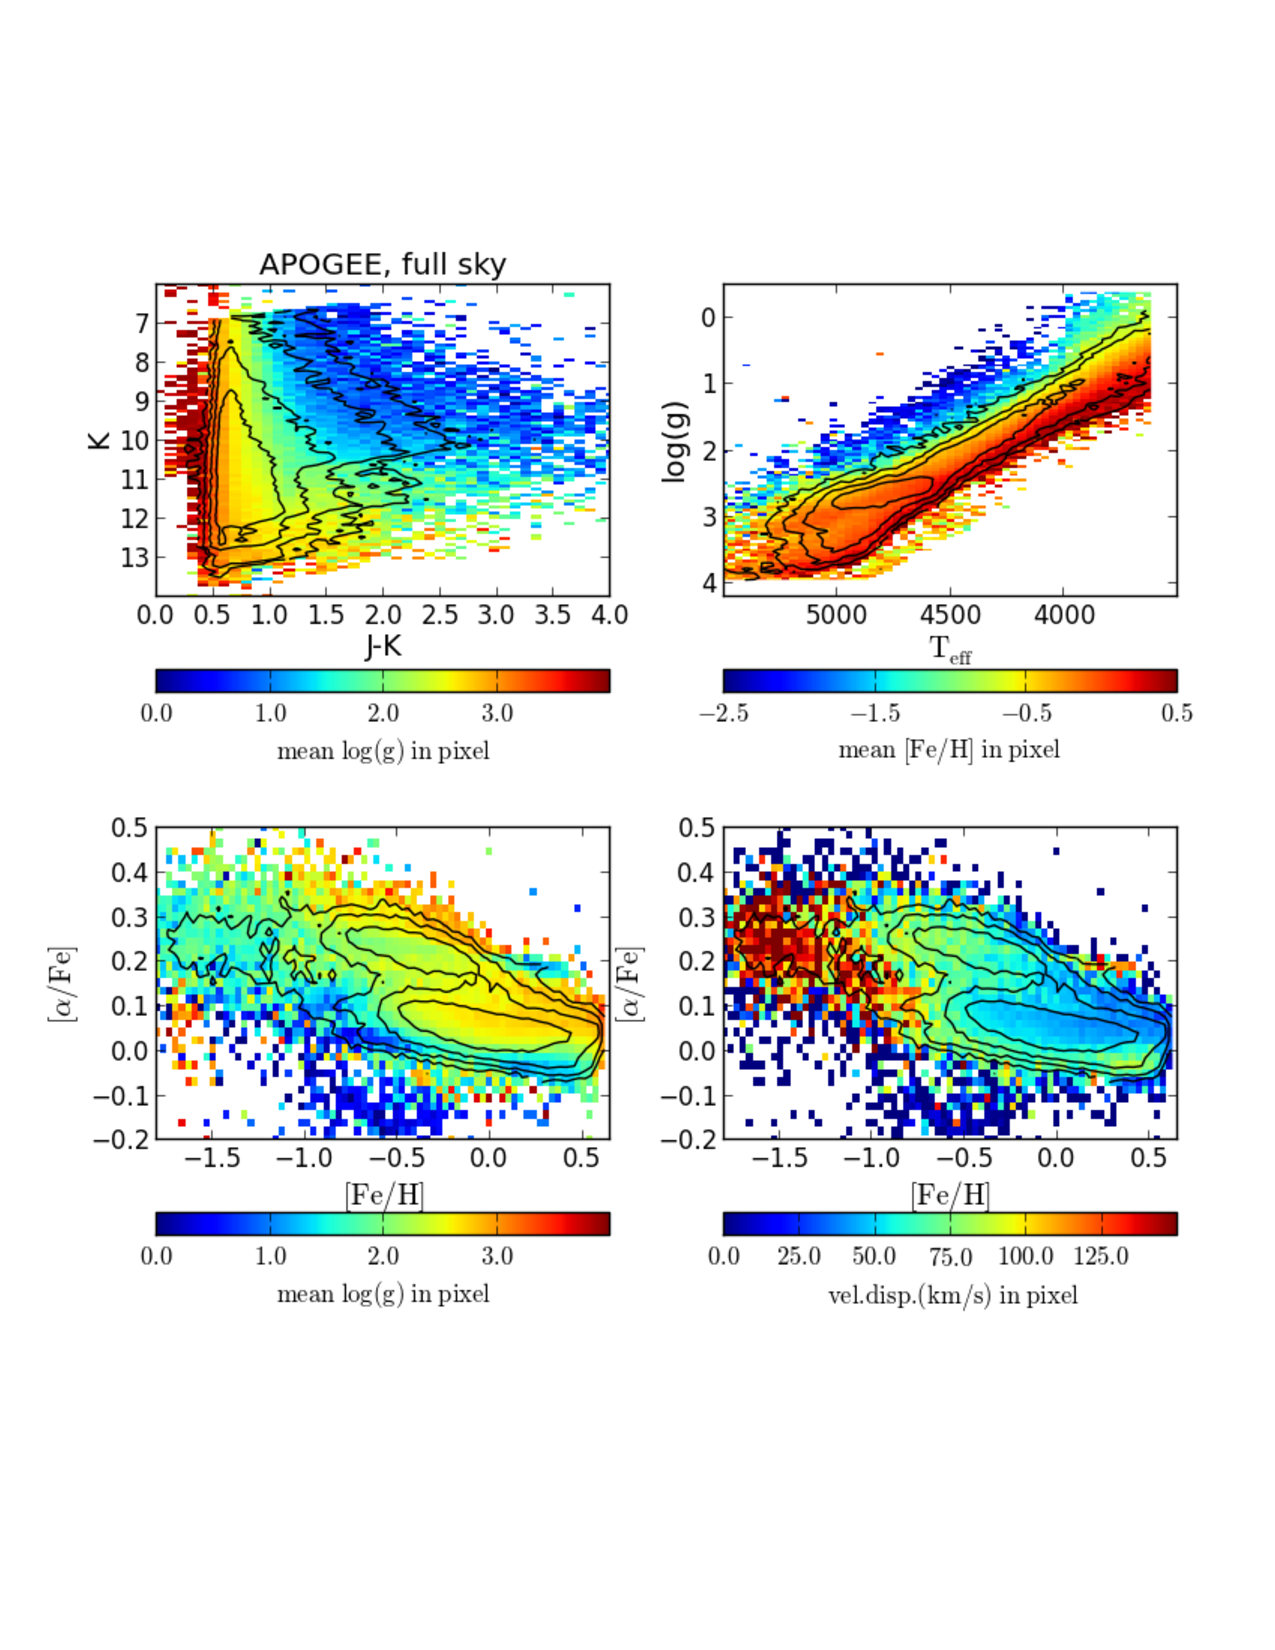
\includegraphics[width=\textwidth]{apogee1.pdf}
  \vskip -1.5in
  \caption{
    This figure was produced with allStarAnalysis1.py. It shows various two-dimensional diagrams  
    for a subset of stars from allStar-v603.fits data file, color-coded using a third quantity marked
    below each panel. 
  }
  \label{basic_example1}
\end{figure}


\begin{figure}
  \centering
  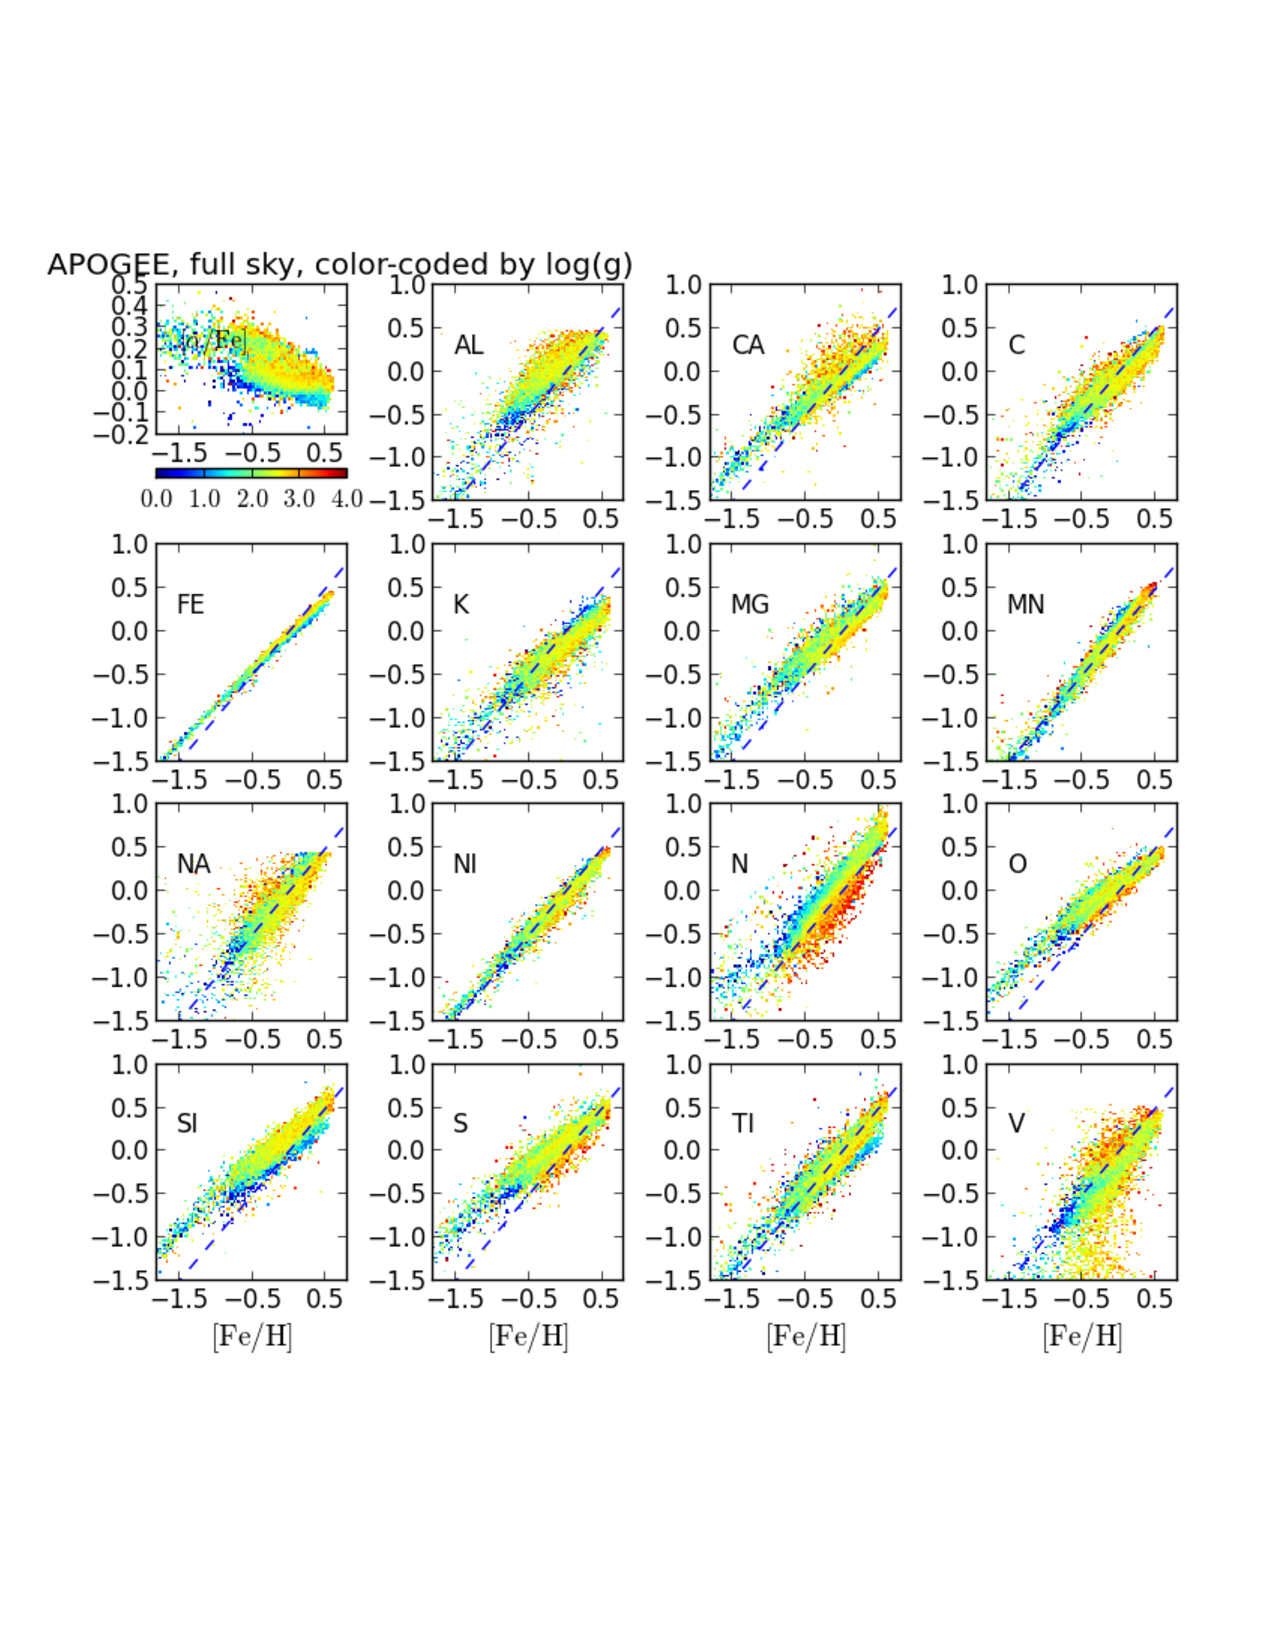
\includegraphics[width=\textwidth]{apogee2.pdf}
  \vskip -1.5in
  \caption{
    This figure was produced with allStarAnalysis2.py. The top left panel shows the $[\alpha/Fe]$ vs. 
$[Fe/H]$ diagram for a subset of stars from allStar-v603.fits data file, color-coded using $log(g)$. 
The remaining 15 panels show the abundances of 15 individual elements, labeled in each panel, 
vs. $[Fe/H]$, using the same color-coding as in the top left panel. 
  }
  \label{basic_example2}
\end{figure}

